\documentclass[12pt,a4paper]{article}

% === PACKAGES ===
\usepackage[utf8]{inputenc}
\usepackage[vietnamese]{babel}
\usepackage{amsmath, amssymb, amsfonts}
\usepackage{graphicx}
\usepackage{booktabs}
\usepackage{caption}
\usepackage{subcaption}
\usepackage{geometry}
\usepackage{hyperref}
\usepackage{cite}
\usepackage{enumitem}
\usepackage{float}

\geometry{margin=2.5cm}
\graphicspath{{figures/}}

% === MATH COMMANDS ===
\newcommand{\R}{\mathbb{R}}
\newcommand{\T}{\mathsf{T}}
\DeclareMathOperator{\diag}{diag}

% ================================================================
\begin{document}

\begin{center}
    {\Large\bfseries BÁO CÁO TIẾN ĐỘ LUẬN VĂN} \\[6pt]
    {\large Phần 1: Cơ sở lý thuyết Actor-Critic ADP \\
    và mô phỏng kiểm chứng trên WMR kinematic} \\[12pt]
    \textbf{Nguyễn Thành Trung} \\
    Chuyên ngành: Điều khiển và Tự động hóa --- GVHD: PGS.TS. Nguyễn Hoài Nam \\
    Đại học Bách khoa Hà Nội --- Tháng 03/2026
\end{center}

\vspace{4pt}\hrule\vspace{8pt}

\noindent\textbf{Công việc đã hoàn thành:}
\begin{enumerate}[nosep]
    \item Nghiên cứu lý thuyết Actor-Critic ADP (Vamvoudakis \& Lewis 2010)
    \item Thiết lập bài toán: động học sai số, hàm cost, phương trình HJB
    \item Implement bộ điều khiển AC-ADP và Backstepping (BC) trên MATLAB
    \item Mô phỏng trên 2 quỹ đạo (tròn, thẳng), so sánh BC / ADP+PE / ADP không PE
    \item Phân tích vai trò PE, hạn chế warm start, dẫn nhập cho SM2
\end{enumerate}

% ================================================================
\section{Bối cảnh lý thuyết: tại sao cần ADP?}

\subsection{Bài toán điều khiển tối ưu phi tuyến}

Xét hệ phi tuyến affine tổng quát:
\begin{equation}\label{eq:nonlinear_sys}
    \dot{x} = f(x) + g(x)\,u, \quad x \in \R^n,\; u \in \R^m
\end{equation}

Ta muốn tìm luật điều khiển $u^*(x)$ cực tiểu hàm cost vô hạn:
\begin{equation}\label{eq:general_cost}
    J(x_0) = \int_0^\infty \big[\, Q(x) + u^\T R\, u \,\big]\, dt, \quad Q(x) \geq 0,\; R > 0
\end{equation}

Hàm giá trị tối ưu $V^*(x) = \min_u J(x)$ thỏa mãn phương trình \textbf{Hamilton-Jacobi-Bellman (HJB)}:
\begin{equation}\label{eq:hjb_general}
    \boxed{0 = Q(x) + {u^*}^\T R\, u^* + \big(\nabla V^*\big)^\T \big[\,f(x) + g(x)\, u^*\,\big]}
\end{equation}
với điều khiển tối ưu:
\begin{equation}\label{eq:optimal_u}
    u^*(x) = -\frac{1}{2} R^{-1}\, g(x)^\T\, \nabla V^*(x)
\end{equation}

\textbf{Vấn đề:} Phương trình HJB (\ref{eq:hjb_general}) là PDE phi tuyến, nói chung \textit{không giải được giải tích} (trừ trường hợp tuyến tính $\to$ Riccati). Đây chính là lý do cần \textbf{Approximate Dynamic Programming (ADP)}: xấp xỉ $V^*(x)$ bằng mạng nơ-ron, rồi học online thông qua dữ liệu.

\subsection{Ý tưởng ADP: xấp xỉ hàm giá trị}

Giả sử $V^*(x)$ có thể biểu diễn (hoặc xấp xỉ) dưới dạng:
\begin{equation}\label{eq:value_approx}
    V^*(x) \approx W^{*\T} \phi(x) + \varepsilon(x)
\end{equation}
với $\phi(x) \in \R^l$ là vector hàm cơ sở (basis), $W^* \in \R^l$ là trọng số tối ưu, $\varepsilon$ là sai số xấp xỉ.

Thay vào (\ref{eq:optimal_u}):
\begin{equation}
    u^* \approx -\frac{1}{2} R^{-1}\, g(x)^\T\, \nabla\phi(x)^\T\, W^*
\end{equation}
với $\nabla\phi = \partial\phi/\partial x \in \R^{l \times n}$ là Jacobian.

\textbf{Bài toán ADP:} Tìm $W^*$ sao cho sai số Bellman $\delta \to 0$. Có hai trường phái chính:
\begin{itemize}
    \item \textbf{Actor-Critic (SM1):} 2 mạng --- Critic ($\hat{W}_c$) xấp xỉ $V$, Actor ($\hat{W}_a$) xấp xỉ $u$. Cập nhật đồng thời.
    \item \textbf{Critic-only (SM2, luận văn):} 1 mạng --- chỉ Critic, chính sách $u$ được suy trực tiếp từ Critic qua (\ref{eq:optimal_u}).
\end{itemize}

% ================================================================
\section{Mô hình WMR và động học sai số}

\subsection{Mô hình kinematic robot vi sai}

Robot di động vi sai (differential-drive WMR) có trạng thái $q = [x, y, \theta]^\T$ (vị trí + hướng trong world frame), đầu vào $u = [v, \omega]^\T$ (vận tốc dài, vận tốc góc):
\begin{equation}\label{eq:kinematics}
    \dot{x} = v\cos\theta, \quad \dot{y} = v\sin\theta, \quad \dot{\theta} = \omega
\end{equation}

Đây là mô hình nonholonomic --- robot không thể dịch ngang, chỉ di chuyển theo hướng $\theta$.

\subsection{Sai số bám trong body frame}

Cho quỹ đạo tham chiếu $q_r(t) = [x_r, y_r, \theta_r]^\T$ sinh bởi $(v_r, \omega_r)$, định nghĩa sai số trong \textit{body frame} của robot (theo Kanayama \cite{Kanayama1990}):
\begin{equation}\label{eq:error_def}
    z = \begin{bmatrix} z_x \\ z_y \\ z_\theta \end{bmatrix}
    = R(\theta)
    \begin{bmatrix} x_r - x \\ y_r - y \\ \theta_r - \theta \end{bmatrix}, \quad
    R(\theta) = \begin{bmatrix}
        \cos\theta & \sin\theta & 0 \\
        -\sin\theta & \cos\theta & 0 \\
        0 & 0 & 1
    \end{bmatrix}
\end{equation}

\textbf{Ý nghĩa vật lý:}
\begin{itemize}[nosep]
    \item $z_x$: sai số dọc (along-track) --- khoảng cách theo hướng robot đang đi
    \item $z_y$: sai số ngang (cross-track) --- robot lệch sang trái/phải bao nhiêu
    \item $z_\theta$: sai số góc --- robot quay sai bao nhiêu so với tham chiếu
\end{itemize}

Dùng body frame (thay vì world frame) vì: (1) các thành phần sai số có ý nghĩa vật lý rõ, (2) phù hợp với cấu trúc nonholonomic, (3) tách biệt feedforward và feedback.

\subsection{Chứng minh động học sai số}

Đặt luật điều khiển tổng quát $u = u_f + u_o$ với:
\begin{itemize}[nosep]
    \item $u_f = [v_r\cos z_\theta,\; \omega_r]^\T$ --- feedforward (bù vận tốc tham chiếu)
    \item $u_o = [u_{o1},\; u_{o2}]^\T$ --- feedback (cần thiết kế)
\end{itemize}

Khi đó $v = v_r\cos z_\theta + u_{o1}$ và $\omega = \omega_r + u_{o2}$. Lấy đạo hàm $z$ theo thời gian (chi tiết dưới đây):

\textbf{Đạo hàm $z_x$:}
\begin{align}
    \dot{z}_x &= \frac{d}{dt}\big[\cos\theta\,(x_r{-}x) + \sin\theta\,(y_r{-}y)\big] \nonumber \\
    &= \omega\, z_y + v_r\cos(\theta_r{-}\theta) - v \nonumber \\
    &= (\omega_r{+}u_{o2})\,z_y + v_r\cos z_\theta - (v_r\cos z_\theta + u_{o1}) \nonumber \\
    &= z_y\,\omega_r \;-\; u_{o1} \;+\; z_y\,u_{o2} \label{eq:dzx}
\end{align}

\textbf{Đạo hàm $z_y$:}
\begin{align}
    \dot{z}_y &= \frac{d}{dt}\big[-\sin\theta\,(x_r{-}x) + \cos\theta\,(y_r{-}y)\big] \nonumber \\
    &= -\omega\, z_x + v_r\sin(\theta_r{-}\theta) \nonumber \\
    &= -(\omega_r{+}u_{o2})\,z_x + v_r\sin z_\theta \nonumber \\
    &= -z_x\,\omega_r + v_r\sin z_\theta \;-\; z_x\,u_{o2} \label{eq:dzy}
\end{align}

\textbf{Đạo hàm $z_\theta$:}
\begin{equation}\label{eq:dzth}
    \dot{z}_\theta = \omega_r - \omega = \omega_r - (\omega_r + u_{o2}) = -u_{o2}
\end{equation}

Viết gọn ở dạng affine:
\begin{equation}\label{eq:error_dynamics}
    \boxed{\dot{z} = f(z, u_r) + g(z)\, u_o}
\end{equation}
với:
\begin{equation}\label{eq:f_and_g}
    f(z, u_r) = \begin{bmatrix} z_y\omega_r \\ -z_x\omega_r + v_r\sin z_\theta \\ 0 \end{bmatrix}, \quad
    g(z) = \begin{bmatrix} -1 & z_y \\ 0 & -z_x \\ 0 & -1 \end{bmatrix}
\end{equation}

\textbf{Điểm then chốt:} Ma trận $g(z)$ phụ thuộc trạng thái $z$ (cụ thể là $z_y, z_x$). Hệ (\ref{eq:error_dynamics}) là \textit{phi tuyến affine}, thuộc đúng dạng (\ref{eq:nonlinear_sys}) $\to$ có thể áp dụng ADP.

\textbf{Lưu ý cấu trúc:}
\begin{itemize}[nosep]
    \item $u_{o1}$ (feedback tốc độ dài) tác động \textit{trực tiếp} lên $\dot{z}_x$ nhưng \textit{không} tác động trực tiếp lên $\dot{z}_y$
    \item $u_{o2}$ (feedback tốc độ góc) tác động lên cả $\dot{z}_x$ (qua $z_y$), $\dot{z}_y$ (qua $-z_x$) và $\dot{z}_\theta$
    \item $z_y$ hội tụ \textit{gián tiếp} thông qua $v_r\sin z_\theta$ --- phải sửa $z_\theta$ trước, $z_y$ mới giảm. Đây là cấu trúc cascade đặc trưng của nonholonomic system.
\end{itemize}

% ================================================================
\section{Actor-Critic ADP --- Lý thuyết chi tiết}

\subsection{Thiết lập bài toán tối ưu}

Áp dụng framework (\ref{eq:general_cost}) cho hệ sai số (\ref{eq:error_dynamics}) với $Q(z) = z^\T Q\, z$:
\begin{equation}\label{eq:cost_wmr}
    J = \int_0^\infty \big( z^\T Q\, z + u_o^\T R\, u_o \big)\, dt, \quad Q = 10\,I_3,\; R = 2\,I_2
\end{equation}

Phương trình HJB trở thành:
\begin{equation}\label{eq:hjb_wmr}
    0 = z^\T Q\, z + {u_o^*}^\T R\, u_o^* + \big(\nabla V^*\big)^\T \big[\,f(z,u_r) + g(z)\, u_o^*\,\big]
\end{equation}

Điều khiển tối ưu:
\begin{equation}\label{eq:u_opt_wmr}
    u_o^* = -\frac{1}{2} R^{-1}\, g(z)^\T\, \nabla V^*(z)
\end{equation}

\subsection{Chọn hàm cơ sở}

Vì $Q(z) = z^\T Q\,z$ là bậc 2, và $V^*$ thường có dạng bậc 2 gần gốc (từ lý thuyết Lyapunov), ta chọn $\phi(z)$ gồm tất cả đơn thức bậc 2 của 3 biến:
\begin{equation}\label{eq:basis}
    \phi(z) = \big[\,z_x^2,\; z_y^2,\; z_\theta^2,\; z_x z_y,\; z_y z_\theta,\; z_x z_\theta\,\big]^\T \in \R^6
\end{equation}

Ma trận Jacobian $\nabla\phi = \partial\phi/\partial z \in \R^{6\times 3}$:
\begin{equation}\label{eq:nabla_phi}
    \nabla\phi = \begin{bmatrix}
        2z_x & 0 & 0 \\
        0 & 2z_y & 0 \\
        0 & 0 & 2z_\theta \\
        z_y & z_x & 0 \\
        0 & z_\theta & z_y \\
        z_\theta & 0 & z_x
    \end{bmatrix}
\end{equation}

Khi đó $\nabla\hat{V} = \nabla\phi^\T \hat{W}$ có kích thước $3\times 1$ (gradient hàm giá trị theo $z$).

\subsection{Cấu trúc Actor-Critic}

\textbf{Critic} xấp xỉ hàm giá trị:
\begin{equation}
    \hat{V}(z) = \hat{W}_c^\T\, \phi(z)
\end{equation}

\textbf{Actor} xấp xỉ chính sách tối ưu (dùng \textit{cùng basis} $\phi$ nhưng \textit{trọng số khác} $\hat{W}_a$):
\begin{equation}\label{eq:actor_policy}
    \hat{u}_o = -\frac{1}{2} R^{-1}\, g(z)^\T\, \nabla\phi^\T\, \hat{W}_a
\end{equation}

Kích thước:
\[
    \underbrace{R^{-1}}_{2\times 2}\; \underbrace{g^\T}_{2\times 3}\; \underbrace{\nabla\phi^\T}_{3\times 6}\; \underbrace{\hat{W}_a}_{6\times 1} = 2\times 1 \quad \checkmark
\]

\textbf{Tại sao cần 2 mạng?} Trong lý thuyết, $\hat{W}_a = \hat{W}_c = W^*$ khi hội tụ. Nhưng nếu chỉ dùng 1 mạng (Critic-only), thì $u_o$ phụ thuộc trực tiếp vào $\hat{W}_c$ đang thay đổi $\to$ tạo vòng feedback giữa policy và value estimation, có thể gây mất ổn định. Actor riêng cho phép tách biệt: Critic học giá trị, Actor học chính sách, hai bên hội tụ dần về nhau.

\subsection{Sai số Bellman và luật cập nhật}

Định nghĩa vector $\sigma$ (``hướng gradient'' trong không gian basis):
\begin{equation}
    \sigma = \nabla\phi\,\big(f + g\,\hat{u}_o\big) \in \R^6
\end{equation}

\textbf{Sai số Bellman} (đo ``khoảng cách'' đến nghiệm HJB):
\begin{equation}\label{eq:bellman_error}
    \delta = \hat{W}_c^\T\, \sigma + z^\T Q\, z + \hat{u}_o^\T R\, \hat{u}_o
\end{equation}

Nếu $\hat{W}_c = W^*$ và $\hat{u}_o = u_o^*$ thì $\delta = 0$ (HJB thỏa mãn đúng).

\textbf{Critic update} (gradient descent trên $\delta$, có $\sigma$-modification \cite{Vamvoudakis2010}):
\begin{equation}\label{eq:critic_law}
    \dot{\hat{W}}_c = -\alpha_c \underbrace{\frac{\sigma}{(1+\sigma^\T\sigma)^2}}_{\bar{\sigma}\text{ (normalized)}} \delta \;-\; \kappa_c\, \hat{W}_c
\end{equation}

\begin{itemize}[nosep]
    \item $\alpha_c = 0.5$: tốc độ học Critic
    \item Chuẩn hóa $(1+\sigma^\T\sigma)^2$: tránh cập nhật quá lớn khi $\sigma$ lớn
    \item $\kappa_c = 0.01$ ($\sigma$-modification): weight decay, chống phát tán trọng số khi $\delta$ không hội tụ hoàn toàn (do sai số xấp xỉ $\varepsilon$)
\end{itemize}

\textbf{Actor update} (Critic đánh giá Actor + kéo Actor về Critic):
\begin{equation}\label{eq:actor_law}
    \dot{\hat{W}}_a = -\alpha_{a1}\, \bar{\sigma}\, e_a \;-\; \alpha_{a2}\,(\hat{W}_a - \hat{W}_c)
\end{equation}
với sai số Actor $e_a = \sigma^\T \hat{W}_c + z^\T Q\, z + \hat{u}_o^\T R\, \hat{u}_o$.

\begin{itemize}[nosep]
    \item Vế 1 ($\alpha_{a1}\,\bar{\sigma}\,e_a$): gradient descent --- Actor giảm sai số Bellman, \textit{dùng trọng số Critic $\hat{W}_c$ để đánh giá} (không dùng $\hat{W}_a$ tự đánh giá mình)
    \item Vế 2 ($\alpha_{a2}(\hat{W}_a - \hat{W}_c)$): kéo $\hat{W}_a \to \hat{W}_c$, đảm bảo Actor và Critic đồng thuận khi hội tụ
    \item $\alpha_{a1} = 0.5$, $\alpha_{a2} = 1.0$
\end{itemize}

\subsection{PE --- Persistence of Excitation}

\textbf{Vấn đề:} Luật cập nhật (\ref{eq:critic_law})--(\ref{eq:actor_law}) chỉ học được khi $\sigma(t)$ ``phong phú'' --- vector $\sigma$ phải quét đủ nhiều hướng trong $\R^6$ theo thời gian. Nếu $z(t)$ hội tụ nhanh về 0 (nhờ feedback tốt), thì $\sigma \to 0$, weights không được cập nhật $\to$ chưa hội tụ đến $W^*$.

\textbf{Điều kiện PE:} Tồn tại $T > 0$, $\mu > 0$ sao cho:
\begin{equation}
    \int_t^{t+T} \bar{\sigma}(\tau)\,\bar{\sigma}(\tau)^\T\, d\tau \geq \mu\, I_6, \quad \forall\, t \geq 0
\end{equation}

Để thỏa mãn, thêm nhiễu kích thích:
\begin{equation}
    n(t) = \sum_{i=1}^{8} A_i \sin(\omega_i\, t)
\end{equation}
với 8 tần số khác nhau (cần $\geq l + 1 = 7$). PE được tắt sau $t_\text{PE} = 30$\,s khi weights đã ổn định.

\subsection{Vấn đề điều kiện ban đầu (warm start)}

\textbf{Nếu $\hat{W}_{c,0} = \hat{W}_{a,0} = 0$:} Actor cho ra $\hat{u}_o = 0$ (không feedback) $\to$ hệ chỉ có feedforward $u_f$ $\to$ sai số $z$ \textit{không hội tụ}, robot trôi xa $\to$ $\phi(z)$ tăng, $\nabla\phi$ tăng $\to$ $\hat{u}_o$ (khi weights bắt đầu thay đổi) tăng rất nhanh $\to$ \textbf{mất ổn định}.

\textbf{Giải pháp:} Khởi tạo $\hat{W}_{c,0} = \hat{W}_{a,0} = [1,1,1,0,0,0]^\T$. Tính $\hat{u}_o$ gần $z = 0$:
\begin{align}
    \nabla\hat{V} &= \nabla\phi^\T\, W_0 = [2z_x,\; 2z_y,\; 2z_\theta]^\T \\
    g^\T\, \nabla\hat{V} &\approx \begin{bmatrix} -1 & 0 & 0 \\ 0 & 0 & -1 \end{bmatrix} \begin{bmatrix} 2z_x \\ 2z_y \\ 2z_\theta \end{bmatrix} = \begin{bmatrix} -2z_x \\ -2z_\theta \end{bmatrix} \quad (\text{khi } z_y \approx 0) \\
    \hat{u}_o &= -\frac{1}{2}\, \frac{1}{2}\,I_2 \begin{bmatrix} -2z_x \\ -2z_\theta \end{bmatrix} = \begin{bmatrix} 0.5\, z_x \\ 0.5\, z_\theta \end{bmatrix}
\end{align}

Đây là P-controller yếu ($K_p = 0.5$): ổn định hệ, nhưng chưa tối ưu $\to$ ADP sẽ cải thiện online.

\textbf{Kết luận quan trọng:} AC-ADP \textit{không thể học từ zero} --- cần ``admissible initial policy'' (chính sách ban đầu ổn định). Đây là hạn chế lý thuyết, không phải lỗi implement.

% ================================================================
\section{Backstepping Controller --- Bộ so sánh}

Bộ điều khiển backstepping \cite{Kanayama1990, Wang2025}:
\begin{equation}\label{eq:bc}
    v = v_r \cos z_\theta + k_1 z_x, \quad \omega = \omega_r + k_2 v_r z_y + k_3 \sin z_\theta
\end{equation}

Suy ra feedback: $u_{o,\text{BC}} = u - u_f = [k_1 z_x,\; k_2 v_r z_y + k_3 \sin z_\theta - k_3 z_\theta + \ldots]$.

BC là \textbf{model-based}, gains $(k_1, k_2, k_3)$ thiết kế trực tiếp từ mô hình $\to$ không cần học, hội tụ ngay. Dùng làm baseline để đánh giá ADP.

% ================================================================
\section{Kết quả mô phỏng}

\subsection{Thiết lập}

\begin{itemize}[nosep]
    \item Tích phân Euler, $\Delta t = 0.001$\,s, $T = 120$\,s
    \item Sai lệch ban đầu: $[0.5,\; -0.3,\; 0.2]$ (m, m, rad)
    \item Quỹ đạo: đường tròn ($R=2$\,m, $v_r=0.3$\,m/s) và đường thẳng ($v_r=0.3$\,m/s)
    \item 3 bộ điều khiển: BC, ADP có PE, ADP không PE
\end{itemize}

\subsection{Bảng kết quả}

\begin{table}[H]
\centering
\caption{So sánh hiệu năng tracking}
\label{tab:results}
\begin{tabular}{llrrr}
\toprule
\textbf{Quỹ đạo} & \textbf{Phương pháp} & $J_c$ & $J_e$ & $z_{\text{rms}}$ \textbf{(10\,s cuối)} \\
\midrule
Circle & BC          &   7.39 &  0.69 & 0.0002 \\
Circle & ADP (PE)    &  17.06 &  1.69 & 0.0004 \\
Circle & ADP (no PE) &  27.96 &  2.77 & 0.0019 \\
\midrule
Line   & BC          &   7.06 &  0.65 & $\approx 0$ \\
Line   & ADP (PE)    & 152.45 & 15.21 & 0.4516 \\
Line   & ADP (no PE) & 114.67 & 11.45 & 0.3608 \\
\bottomrule
\end{tabular}
\end{table}

\noindent $J_c = \int (z^\T Qz + u_o^\T Ru_o)\,dt$, \;$J_e = \int \|z\|^2 dt$, \;$z_\text{rms}$: RMS sai số trong 10\,s cuối.

\subsection{Phân tích kết quả trên đường tròn}

\begin{figure}[H]
\centering
\begin{minipage}{0.48\textwidth}
    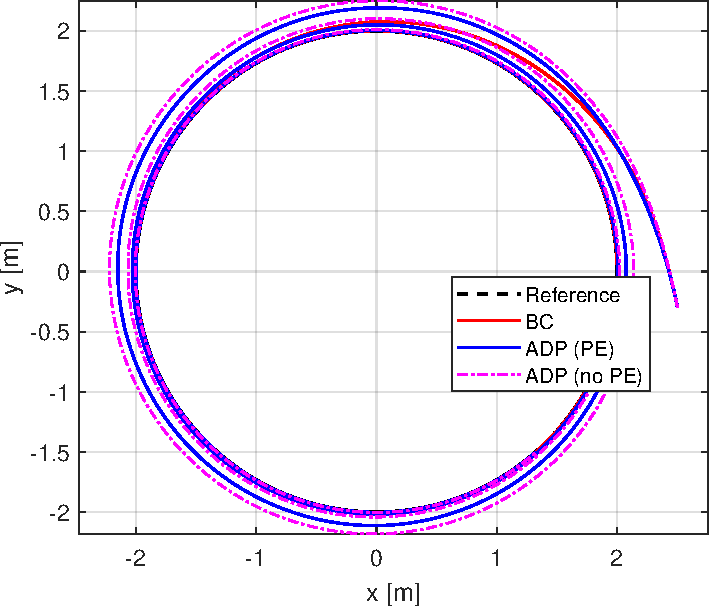
\includegraphics[width=\textwidth]{xy_circle.pdf}
    \caption{Quỹ đạo XY --- Circle}
    \label{fig:xy_circle}
\end{minipage}\hfill
\begin{minipage}{0.48\textwidth}
    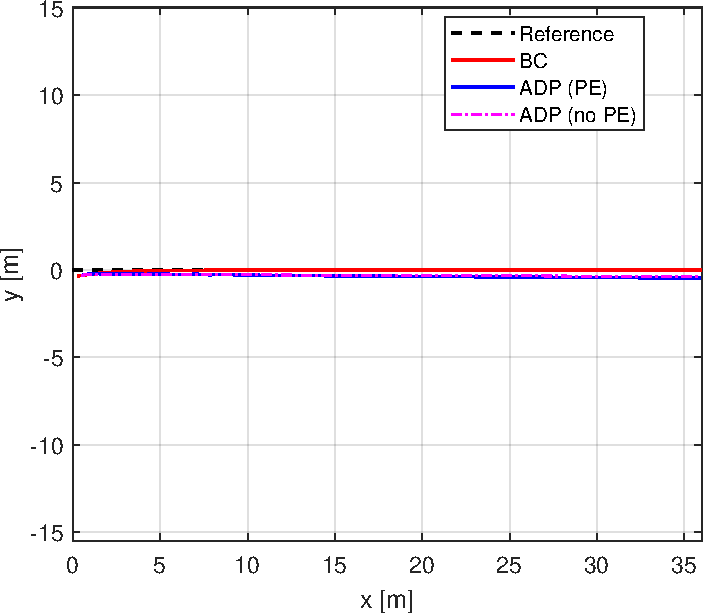
\includegraphics[width=\textwidth]{xy_line.pdf}
    \caption{Quỹ đạo XY --- Line}
    \label{fig:xy_line}
\end{minipage}
\end{figure}

\begin{figure}[H]
\centering
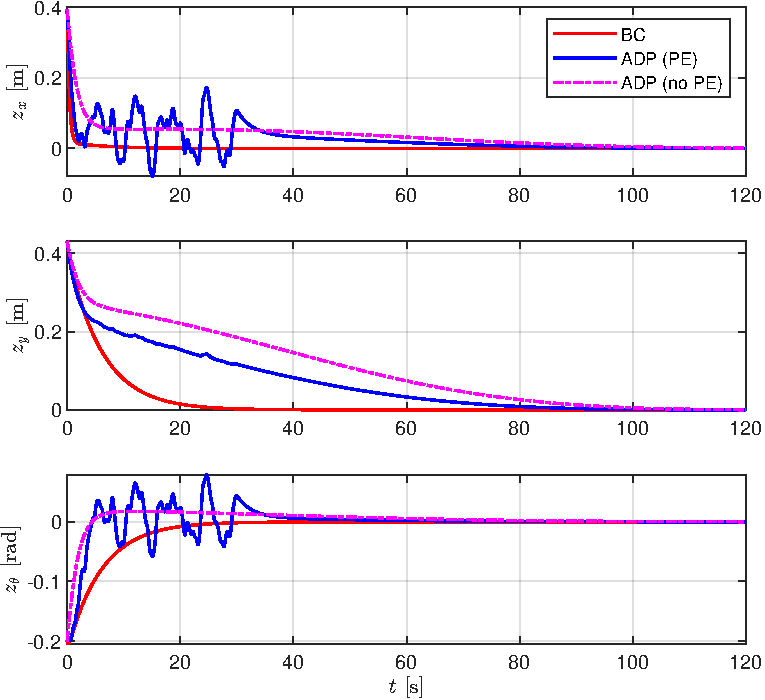
\includegraphics[width=0.85\textwidth]{error_circle.pdf}
\caption{Sai số $z(t)$ trên đường tròn --- BC (đỏ), ADP+PE (xanh), ADP no-PE (tím).}
\label{fig:error_circle}
\end{figure}

\textbf{Quan sát:}
\begin{enumerate}[nosep]
    \item BC hội tụ nhanh nhất ($J_c = 7.39$, $z_\text{rms} \approx 0$) --- dễ hiểu vì gains tối ưu sẵn.
    \item ADP+PE: $z_\text{rms} = 0.0004$\,m (gần hoàn hảo), nhưng $J_c = 17.06$ (gấp $2.3\times$) --- chi phí phần lớn nằm ở 30\,s đầu (PE + chưa hội tụ).
    \item ADP no-PE: $J_c = 27.96$ (gấp $1.6\times$ so với có PE) $\Rightarrow$ \textbf{PE thực sự giúp ADP học tốt hơn trên đường tròn}.
    \item Giải thích: $\omega_r = 0.15$\,rad/s $\neq 0$ trên đường tròn tạo coupling trong drift $f$ $\to$ hệ có kích thích tự nhiên, PE bổ sung thêm.
\end{enumerate}

\subsection{Phân tích kết quả trên đường thẳng}

\begin{figure}[H]
\centering
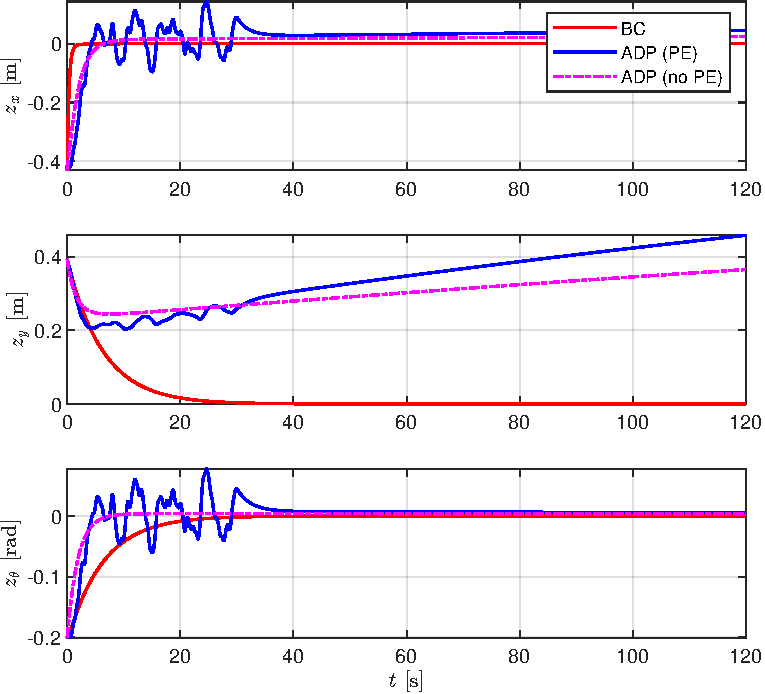
\includegraphics[width=0.85\textwidth]{error_line.pdf}
\caption{Sai số $z(t)$ trên đường thẳng.}
\label{fig:error_line}
\end{figure}

\textbf{Quan sát bất ngờ:} ADP no-PE \textit{tốt hơn} ADP+PE ($J_c = 115$ vs.\ $152$).

\textbf{Giải thích:} Trên đường thẳng ($\omega_r = 0$), drift $f = [0,\; v_r\sin z_\theta,\; 0]^\T$ --- không có coupling $z_x$-$z_y$ qua $\omega_r$. PE ngoài thêm nhiễu làm tăng cost mà không cải thiện quality of exploration trên các mode đã đủ excite.

\subsection{Hội tụ trọng số}

\begin{figure}[H]
\centering
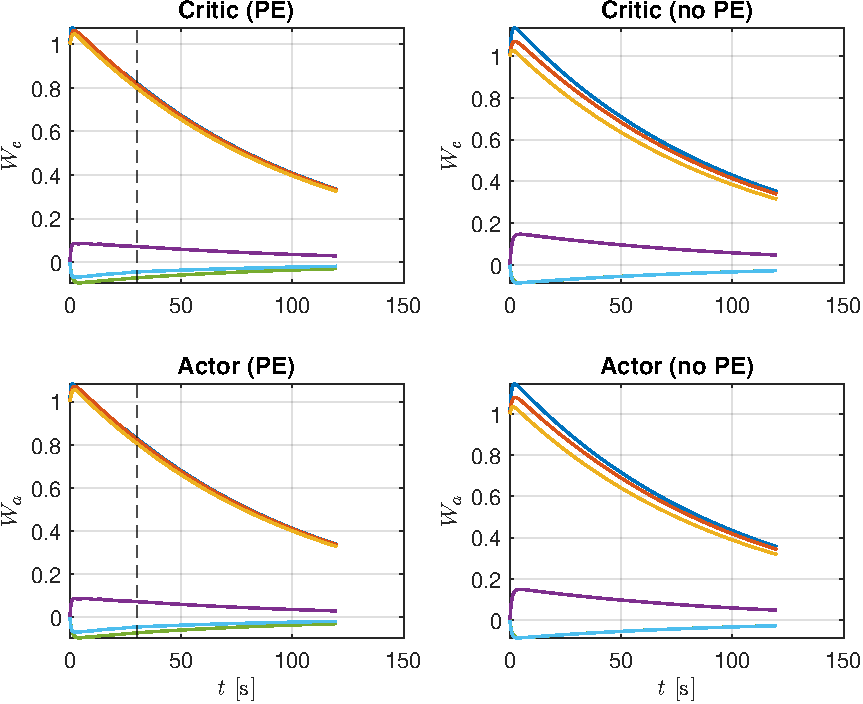
\includegraphics[width=0.88\textwidth]{weights_comparison.pdf}
\caption{Trọng số $\hat{W}_c$ và $\hat{W}_a$ trên quỹ đạo tròn: PE (trái) vs.\ no PE (phải).}
\label{fig:weights}
\end{figure}

\begin{figure}[H]
\centering
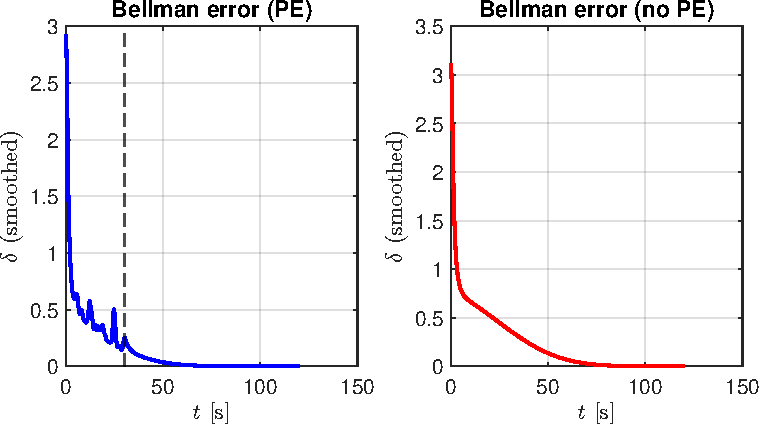
\includegraphics[width=0.85\textwidth]{bellman_error.pdf}
\caption{Sai số Bellman $\delta(t)$ --- PE (trái) vs.\ no PE (phải).}
\label{fig:bellman}
\end{figure}

% ================================================================
\section{Tổng hợp: hạn chế AC-ADP và hướng đi SM2}

\begin{enumerate}
    \item \textbf{Cần warm start:} $W_0 = 0 \to$ mất ổn định. AC-ADP đòi hỏi chính sách ban đầu admissible.

    \item \textbf{PE phụ thuộc quỹ đạo:} giúp trên circle ($\omega_r \neq 0$) nhưng phản tác dụng trên line ($\omega_r = 0$). Không có tiêu chí chọn PE tổng quát.

    \item \textbf{2 mạng, nhiều siêu tham số:} $\alpha_c, \alpha_{a1}, \alpha_{a2}, \kappa_c$, PE amplitudes/frequencies/$t_\text{PE}$ --- rất nhạy cảm, tuning thủ công.

    \item \textbf{Hội tụ chậm:} đường thẳng vẫn $z_\text{rms} = 0.36$\,m sau 120\,s.
\end{enumerate}

\textbf{SM2 (Critic-only + Concurrent Learning)} sẽ khắc phục:
\begin{itemize}[nosep]
    \item \textbf{1 mạng} Critic duy nhất, $u_o$ suy trực tiếp $\to$ ít tham số, bỏ Actor update
    \item \textbf{Concurrent Learning:} lưu history stack $\{z_k, \sigma_k\}$, dùng lại dữ liệu cũ $\to$ \textit{thay thế PE hoàn toàn}
    \item Hội tụ exponential (có chứng minh Lyapunov) thay vì asymptotic
\end{itemize}

% ================================================================
\begin{thebibliography}{9}

\bibitem{Wang2025}
Y.~Wang, Z.~Li, et al.,
``Adaptive dynamic programming-based fixed-time optimal control for wheeled mobile robot,''
\textit{IEEE Robotics and Automation Letters}, vol.~10, no.~1, pp.~176--183, Jan. 2025.

\bibitem{Vamvoudakis2010}
K.~G.~Vamvoudakis and F.~L.~Lewis,
``Online actor-critic algorithm to solve the continuous-time infinite horizon optimal control problem,''
\textit{Automatica}, vol.~46, no.~5, pp.~878--888, 2010.

\bibitem{Kanayama1990}
Y.~Kanayama, Y.~Kimura, F.~Miyazaki, and T.~Noguchi,
``A stable tracking control method for an autonomous mobile robot,''
in \textit{Proc. IEEE Int. Conf. Robotics and Automation}, 1990, pp.~384--389.

\bibitem{Fierro1997}
R.~Fierro and F.~L.~Lewis,
``Control of a nonholonomic mobile robot: backstepping kinematics into dynamics,''
\textit{J. Robotic Systems}, vol.~14, no.~3, pp.~149--163, 1997.

\end{thebibliography}

\end{document}
